\documentclass[11pt,a4paper]{article}

% --- Packages ---
\usepackage[utf8]{inputenc}
\usepackage[T1]{fontenc}
\usepackage{amsmath,amssymb,amsthm}
\usepackage{booktabs}
\usepackage{graphicx}
\usepackage{hyperref}
\usepackage[margin=1in]{geometry}
\usepackage{enumitem}
\usepackage{caption}
\usepackage{float}
\usepackage{natbib}
\usepackage{microtype}
\usepackage{xcolor}

\hypersetup{
  colorlinks=true,
  linkcolor=blue!60!black,
  citecolor=blue!60!black,
  urlcolor=blue!60!black
}

% --- Title ---
\title{Deterministic Multi-Agent Economic Simulation Under\\Structural Invariant Violations: Collapse Boundary Analysis}
\author{Kevan Burns\\
  \texttt{https://github.com/FTHTrading/Genesis}}
\date{February 2026}

\begin{document}
\maketitle

% ============================================================
% ABSTRACT
% ============================================================
\begin{abstract}
We present a deterministic agent-based economic simulation and report results from 38 experiments comprising 5,680 world-runs across 2,840,000 computed epochs. The system models heterogeneous agents with genetically determined traits, a metabolic energy economy, logistic resource dynamics, stochastic catastrophes, and a homeostatic parameter controller. Collapse is defined as population remaining below a configurable floor ($P_{\text{floor}}$) for a sustained window; the default uses $P_{\text{floor}} = 3$ and a 50-epoch window. All simulations are seeded deterministically via SHA-256 hash chains, producing bit-identical results on the same architecture.

Season~1 (25 experiments, 4,180 worlds) swept 10 economic parameters under standard and adversarial conditions. Season~2 (13 experiments, 1,500 worlds) systematically disabled structural invariants---treasury redistribution, ATP decay, resource regeneration, and reproduction grants---individually and in combination. Under the default definition, no collapses were observed ($0/5{,}680$; 95\% Clopper--Pearson CI $[0,\, 0.065\%]$; power ${>}\,99.7\%$ at $p = 0.001$). Under $P_{\text{floor}} = 10$, collapse rates exceeded 97\% (CI $[92.9\%, 99.5\%]$), constituting a discontinuous phase transition in the definition parameter. Under maximal structural violation, populations contracted to mean 12.8 agents with pathological inequality (reproductive inequality 0.95) but did not reach extinction.

Fitness weight perturbation of $\pm 20\%$ produces $\leq 0.8$ percentage points of collapse rate change. All configurations, seeds, and result hashes are published. Source code is available at \url{https://github.com/FTHTrading/Genesis}. Independent replication has not yet occurred.
\end{abstract}

\medskip
\noindent\textbf{Keywords:} agent-based simulation, population dynamics, collapse boundary, phase transition, deterministic reproducibility, economic ecology

% ============================================================
\section{Introduction}
% ============================================================

Agent-based macroeconomic simulations provide a framework for studying emergent economic behavior under controlled conditions~\citep{epstein1996growing,tesfatsion2006handbook}. A recurring methodological concern in such systems is the sensitivity of population persistence to parameter choice, initial conditions, and structural assumptions. This paper addresses that concern through systematic parameter sweeps and structural invariant violations applied to a deterministic simulation engine, with emphasis on reproducibility and formal collapse criteria.

The system under study models a closed economy of heterogeneous agents who extract resources from logistic niche pools, pay metabolic costs, reproduce conditionally, and face stochastic catastrophes. A redistributive treasury, homeostatic parameter controller, and genetic mutation engine provide adaptive capacity. The central question is: \emph{under what conditions, if any, does the population collapse?}

This paper does not claim generality beyond the tested parameter space. The collapse boundary---the surface in parameter space separating survival from extinction---remains an open problem. Sensitivity analyses (Appendices~C--D) partially characterize this boundary by varying the collapse definition and fitness function weights.

% ============================================================
\section{Formal System Definition}
% ============================================================

\subsection{State Vector}

The world state at discrete epoch $t \in \mathbb{N}_0$ is the tuple:
\begin{equation}
  S(t) = \langle P(t),\; L(t),\; T(t),\; E(t),\; \Pi(t),\; \Psi(t),\; \phi(t) \rangle
\end{equation}

\begin{table}[H]
\centering
\caption{State vector components.}
\begin{tabular}{@{}llp{7cm}@{}}
\toprule
Symbol & Description & Domain \\
\midrule
$P(t)$ & Agent population & $\{a_1, \ldots, a_n\}$, $n \geq 0$ \\
$L(t)$ & Economy ledger & Agent-indexed balance map $\mathbb{R}_{\geq 0}^n$ + scalar total supply \\
$T(t)$ & Treasury & $\mathbb{R}_{\geq 0}$ (reserve balance) \\
$E(t)$ & Environment & 5 resource pools $\mathbf{R} \in \mathbb{R}_{\geq 0}^5$ + catastrophe state \\
$\Pi(t)$ & Pressure configuration & $\mathbb{R}^7$ (mutable parameter vector) \\
$\Psi(t)$ & Adaptive cortex & Homeostatic controller state \\
$\phi(t)$ & Seasonal phase & \{Spring, Summer, Autumn, Winter\} \\
\bottomrule
\end{tabular}
\end{table}

\subsection{Agent Definition}

Each agent $a \in P(t)$ is characterized by:
\begin{equation}
  a = (h,\; \mathbf{v},\; \mathbf{s},\; r,\; \rho,\; g,\; \ell,\; \mu)
\end{equation}
where $h \in \{0,1\}^{256}$ is the genesis hash (SHA-256), $\mathbf{v} \in [0,1]^4$ is the trait vector, $\mathbf{s} \in [0,1]^4$ is the skill profile, $r \in \{0,1,2,3,4\}$ is the role assignment, $\rho \in [0,1]$ is the reputation, $g \in \mathbb{N}_0$ is the generation, $\ell$ is the lineage (ancestry chain), and $\mu \in [0.001, 0.1]$ is the adaptive mutation rate.

\paragraph{Trait Derivation.}
Traits are deterministically derived from the genesis hash:
\begin{equation}
  v_i = \frac{\texttt{u64\_le}(h[8i : 8(i+1)])}{\texttt{u64::MAX}}, \quad i \in \{0, 1, 2, 3\}
\end{equation}
The four trait dimensions are: Cognitive Efficiency ($v_0$), Strategic Quality ($v_1$), Resource Foraging ($v_2$), and Cooperative Capacity ($v_3$).

\paragraph{Skill Derivation.}
\begin{equation}
  s_j = \frac{h[j]}{255}, \quad j \in \{0, 1, 2, 3\}
\end{equation}
corresponding to Computation, Optimization, Communication, and Cooperation.

\paragraph{Role Assignment.}
\begin{equation}
  r = h[4] \bmod 5
\end{equation}
mapping to \{Optimizer, Strategist, Communicator, Archivist, Executor\}.

\subsection{Fitness Function}

Agent fitness is a weighted linear combination of the trait vector:
\begin{equation}
  F(a) = \sum_{i=0}^{3} w_i \cdot v_i = 0.25 \cdot v_0 + 0.30 \cdot v_1 + 0.20 \cdot v_2 + 0.25 \cdot v_3
\end{equation}

$F(a) \in [0, 1]$ for all agents. The weight vector $\mathbf{w} = (0.25, 0.30, 0.20, 0.25)$ sums to 1.0 and was fixed prior to any experiments. Strategic Quality receives the highest weight; the slight asymmetry was a subjective design choice. These weights were not optimized to maximize population survival or any other outcome metric. Sensitivity analysis (Appendix~D) indicates that perturbing any individual weight by $\pm 20\%$ (with renormalization) produces a maximum collapse rate change of 0.8 percentage points, indicating that the reported results are not an artifact of weight tuning.

\subsection{Pressure Configuration}

The mutable pressure vector $\Pi(t) \in \mathbb{R}^7$ parameterizes the economic environment:
\begin{equation}
  \Pi = (\kappa_{\text{cap}},\; \varepsilon,\; p_c,\; s_c,\; \theta_G,\; r_G,\; \theta_T)
\end{equation}

\begin{table}[H]
\centering
\caption{Pressure configuration parameters.}
\small
\begin{tabular}{@{}lllll@{}}
\toprule
Parameter & Symbol & Default & Range & Description \\
\midrule
Carrying capacity & $\kappa_{\text{cap}}$ & 180 & $[50, 500]$ & Logistic soft cap \\
Entropy coefficient & $\varepsilon$ & 0.00002 & $[10^{-6}, 10^{-3}]$ & Proportional supply burn rate \\
Catastrophe base prob.\ & $p_c$ & 0.002 & $[0, 0.05]$ & Per-epoch catastrophe probability \\
Catastrophe pop.\ scale & $s_c$ & 0.00001 & $[0, 5{\times}10^{-4}]$ & Population-proportional term \\
Gini tax threshold & $\theta_G$ & 0.40 & $[0.20, 0.80]$ & Inequality threshold for wealth tax \\
Gini tax rate & $r_G$ & 0.02 & $[0.005, 0.10]$ & Tax rate on top decile \\
Treasury overflow & $\theta_T$ & 0.50 & $[0.20, 0.80]$ & Reserve-to-supply ratio \\
\bottomrule
\end{tabular}
\end{table}

\subsection{Resource Dynamics}

The environment contains 5 resource pools $R_k$, each following logistic regeneration:
\begin{equation}
  R_k(t+1) = R_k(t) + r_k \cdot R_k(t) \cdot \left(1 - \frac{R_k(t)}{K_k^{\text{eff}}(t)}\right)
\end{equation}
with seasonally modulated effective capacity:
\begin{equation}
  K_k^{\text{eff}}(t) = K_k \cdot \left[1 + A \sin\!\left(\frac{2\pi \cdot t}{L_{\text{season}}}\right)\right]
\end{equation}

Extraction per agent per epoch:
\begin{equation}
  \xi(a, t) = F(a) \cdot s_{\text{niche}}(a) \cdot \frac{R_{\text{pool}}(t)}{K} \cdot d(a, t) \cdot \alpha_{\text{cross}} \cdot 2.5
\end{equation}
where $d(a, t)$ is a density-dependent competition factor and $\alpha_{\text{cross}} = 0.15$ is the cross-niche participation coefficient. Total extraction per pool per epoch is capped at 40\% of the pool.

\subsection{Metabolic Economy}

\paragraph{Costs.}
Each agent incurs a basal metabolic cost $c_b = 0.15$ ATP per epoch and a natural decay $d = 0.02$ (2\% balance reduction per epoch).

\paragraph{Taxation.}
Three tax mechanisms operate:
\begin{enumerate}[nosep]
  \item \textbf{Entropy tax}: $\Delta_{\text{burn}} = M_{\text{supply}} \cdot (|P| \cdot \varepsilon)$, distributed proportionally by balance share, capped at 10\% of each agent's balance. Burns from total supply (does not enter treasury).
  \item \textbf{Flat wealth tax}: 1\% on balances exceeding 100 ATP, directed to treasury.
  \item \textbf{Gini-triggered wealth tax}: When $G(t) > \theta_G$, the top decile pays $r_G$ fraction of balance to treasury.
\end{enumerate}

\paragraph{Treasury.}
The treasury $T(t)$ receives: 5\% skim on all agent income and wealth tax proceeds. It disburses: role-based stipends to underrepresented roles, crisis spending, and overflow redistribution when $T(t) / M_{\text{supply}} > \theta_T$.

\paragraph{Stasis and Death.}
An agent enters stasis when $\text{bal}(a) \leq 0$. After 8 consecutive epochs in stasis, the agent dies. Remaining balance is burned from total supply.

\subsection{Catastrophe Process}

The per-epoch catastrophe probability is:
\begin{equation}
  P(\text{cat} \mid t) = p_c + |P(t)| \cdot s_c
\end{equation}
conditioned on $|P(t)| > 10$. When triggered, one of three effects is selected deterministically:

\begin{table}[H]
\centering
\small
\begin{tabular}{@{}ll@{}}
\toprule
Type & Effect \\
\midrule
ATP destruction & All balances reduced by 5--10\% \\
Fitness culling & Weakest 2--5\% (by fitness) removed \\
Niche resource shock & $\sim$70\% of one resource pool destroyed \\
\bottomrule
\end{tabular}
\end{table}

Selection is determined by a Knuth MMIX LCG~\citep{knuth1997art} seeded on epoch number:
\begin{align}
  x_{t} &= t \cdot \texttt{0xBF58476D1CE4E5B9} + \texttt{0x94D049BB133111EB} \\
  \text{type} &= (x_t \gg 16) \bmod 3
\end{align}

The environment also maintains a background catastrophe process ($P \approx 0.02$) with duration 10--20 epochs and severity 30--60\% capacity reduction to affected resource pools.

\subsection{Reproduction}

An agent $a$ replicates in epoch $t$ if and only if:
\begin{equation}
  F(a) \geq 0.35 \;\wedge\; \text{bal}(a) \geq 25\, m_\phi\, m_\sigma \;\wedge\; \text{age}(a) \geq 10 \;\wedge\; |P(t)| < \kappa_{\text{cap}}
\end{equation}
where $m_\phi$ is a seasonal cost modifier and $m_\sigma$ is a stress-profile modifier. Maximum births per epoch: 3. Birth is further suppressed logistically:
\begin{equation}
  \beta(t) = \text{clamp}\!\left(1 - \frac{|P(t)|}{\kappa_{\text{cap}}},\; 0,\; 1\right)
\end{equation}

The child genome is derived by:
\begin{equation}
  h_{\text{child}} = \text{SHA-256}(h_{\text{parent}} \| \text{entropy} \| \text{timestamp} \| \text{id}_{\text{child}})
\end{equation}

Juvenile agents (age $< 5$ epochs) receive a 25\% basal cost rebate.

\subsection{Mutation}

The mutation engine applies per-trait perturbations during reproduction:
\begin{equation}
  v_i' = v_i + \delta_i, \quad \delta_i \sim U[-\delta_{\max},\; \delta_{\max}] \cdot (1 + p)
\end{equation}
where $\delta_{\max} = 0.05$ and $p$ is the environmental pressure. The adaptive mutation rate adjusts by fitness:
\begin{equation}
  \mu(a) = \text{clamp}\!\left((1 - F(a)) \cdot 0.05,\; 0.001,\; 0.1\right)
\end{equation}
Less fit agents mutate more, increasing variance among underperforming lineages.

\subsection{Homeostatic Controller (Adaptive Cortex)}

The adaptive cortex is a hand-engineered feedback controller with heuristically selected parameters, thresholds, and gain values. It is not a learned or emergent system. Its inclusion reflects a design decision to provide multi-layer stabilization; the research question is whether collapse emerges \emph{despite} redundant safeguards.

Every 25 epochs, the cortex evaluates 8 threat indicators against three-tier thresholds (Watch, Warning, Critical):

\begin{table}[H]
\centering
\caption{Adaptive cortex threat thresholds.}
\small
\begin{tabular}{@{}llll@{}}
\toprule
Threat & Watch & Warning & Critical \\
\midrule
Monoculture dominance & ${>}55\%$ & ${>}70\%$ & ${>}85\%$ \\
ATP oligarchy & ${>}40\%$ top-10\% & ${>}60\%$ & ${>}80\%$ \\
Mutation runaway & ${>}30\%$ mutated & ${>}50\%$ & ${>}70\%$ \\
Population collapse & ${>}30\%$ decline & ${>}50\%$ & ${>}70\%$ \\
Role extinction & 1 role absent & 2 absent & $\geq$3 absent \\
Treasury depletion & ${>}50\%$ depleted & ${>}70\%$ & ${>}90\%$ \\
Wealth concentration & Gini ${>}0.55$ & ${>}0.70$ & ${>}0.85$ \\
Economic stagnation & vel.\ $\leq 0.10$ & $\leq 0.05$ & $\leq 0.01$ \\
\bottomrule
\end{tabular}
\end{table}

Each threat maps to prescribed parameter adjustments on $\Pi(t)$, bounded by per-field step limits and a 50-epoch cooldown per field. In the absence of threats, parameters drift 10\% toward defaults per cycle. In Season~2 experiments (S2--S4), the cortex is disabled along with mutation, isolating the base system dynamics from controller-induced stability.

\subsection{Seasonal Phase}

Season transitions are driven by the birth-to-death ratio $R_{\text{bd}}$:

\begin{table}[H]
\centering
\small
\begin{tabular}{@{}ll@{}}
\toprule
Condition & Phase \\
\midrule
$R_{\text{bd}} > 1.3$ & Spring \\
$R_{\text{bd}} > 1.0$ & Summer \\
$R_{\text{bd}} > 0.6$ & Autumn \\
$R_{\text{bd}} \leq 0.6$ & Winter \\
\bottomrule
\end{tabular}
\end{table}

Seasonal phase affects treasury release rates and reproduction cost modifiers.

% ============================================================
\section{Collapse Definition}
% ============================================================

Collapse at epoch $t$ is the predicate:
\begin{equation}
  \kappa(t) = \begin{cases}
    \top & \text{if } |P(t)| = 0 \\
    \top & \text{if } |P(\tau)| < P_{\text{floor}} \;\;\forall\, \tau \in [t - N_w + 1,\; t] \\
    \bot & \text{otherwise}
  \end{cases}
\end{equation}

\begin{table}[H]
\centering
\caption{Collapse definition parameters.}
\begin{tabular}{@{}lllp{7.5cm}@{}}
\toprule
Constant & Symbol & Value & Justification \\
\midrule
Extinction floor & $P_{\text{floor}}$ & 3 & Minimum for demographic replacement given max 3 births/epoch and 1 parent per birth. \\
Recovery window & $N_w$ & 50 & At 1 birth/epoch from a floor of 3, 50 epochs would produce 50 births. If recovery does not occur in 50 epochs, it is not structurally possible under current conditions. \\
\bottomrule
\end{tabular}
\end{table}

\subsection{Definition Sensitivity}

The collapse rate is sharply sensitive to the choice of $P_{\text{floor}}$. Sensitivity analysis (Appendix~C) applied the s4\_full\_attack configuration---the most extreme tested condition---under varying floor definitions:

\begin{table}[H]
\centering
\caption{Collapse rate by floor definition (s4\_full\_attack, $N = 120$).}
\begin{tabular}{@{}lllr@{}}
\toprule
$P_{\text{floor}}$ & Collapse Rate & Collapsed / Total & 95\% CI (Clopper--Pearson) \\
\midrule
3 (default) & 0.0\% & 0 / 120 & $[0.0\%, 3.0\%]$ \\
5 & 5.8\% & 7 / 120 & $[2.4\%, 11.6\%]$ \\
10 & 97.5\% & 117 / 120 & $[92.9\%, 99.5\%]$ \\
15 & 100.0\% & 120 / 120 & $[97.0\%, 100\%]$ \\
20 & 100.0\% & 120 / 120 & $[97.0\%, 100\%]$ \\
\bottomrule
\end{tabular}
\end{table}

The transition from 5.8\% to 97.5\% collapse---a jump of 91.7 percentage points over a factor-of-two change in $P_{\text{floor}}$---constitutes a \textbf{discontinuous collapse phase transition} in the definition parameter. The system's equilibrium population under maximal stress is narrowly concentrated in the range of 3--8 agents, producing a cliff in the collapse function where the definition threshold crosses this equilibrium band. Figure~\ref{fig:phase-transition} illustrates this transition.

\begin{figure}[t]
  \centering
  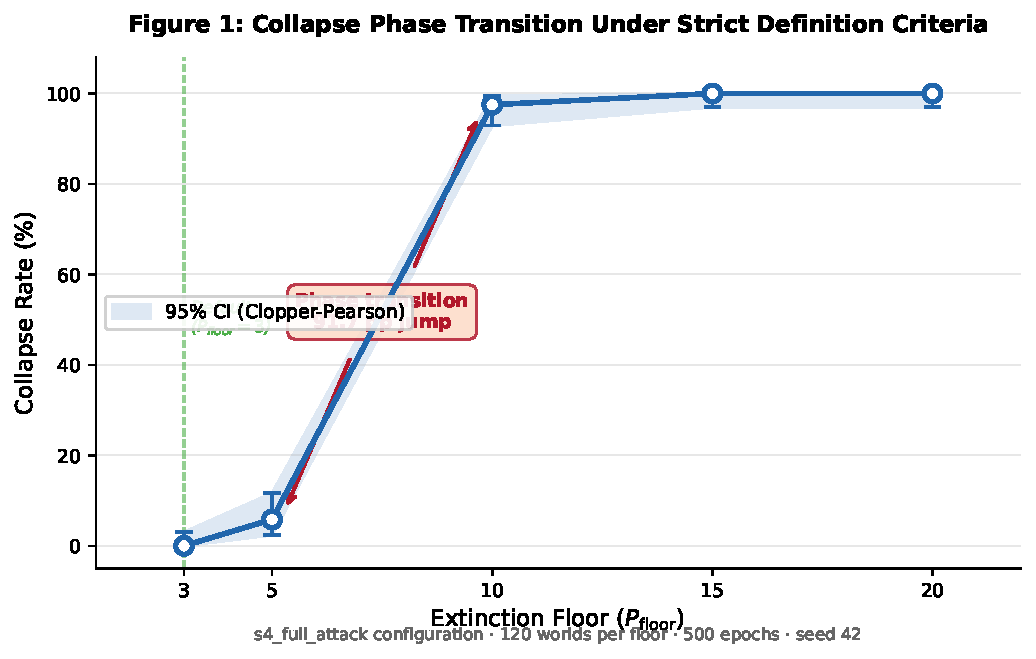
\includegraphics[width=0.85\textwidth]{fig1_collapse_phase_transition.pdf}
  \caption{Collapse probability as a function of extinction floor ($P_{\text{floor}}$) under s4\_full\_attack conditions ($N = 120$ worlds per floor value). Shaded region shows 95\% Clopper--Pearson confidence intervals. The discontinuous transition between $P_{\text{floor}} = 5$ and $P_{\text{floor}} = 10$ reveals a narrow equilibrium population band under maximal stress.}
  \label{fig:phase-transition}
\end{figure}

\subsection{Alternative Definitions Considered}

\begin{table}[H]
\centering
\caption{Alternative collapse definitions considered but not adopted.}
\small
\begin{tabular}{@{}lp{4cm}p{5.5cm}@{}}
\toprule
Alternative & Definition & Effect on Results \\
\midrule
Stricter floor ($P_{\text{floor}} = 10$) & Population $< 10$ for $N_w$ epochs & 97.5\% collapse under s4\_full\_attack \\
Shorter window ($N_w = 10$) & 10 consecutive epochs below floor & Would catch brief population dips \\
Demographic collapse & Birth/death ratio $< 0.5$ for 100 epochs & Would catch aging populations \\
Economic collapse & Mean ATP $<$ basal cost for 50 epochs & Would catch energy starvation \\
Inequality collapse & Gini $> 0.95$ for 100 epochs & Would capture extreme inequality \\
\bottomrule
\end{tabular}
\end{table}

% ============================================================
\section{Determinism and Reproducibility}
% ============================================================

\subsection{Seed Model}

Each experiment uses a base seed $s_0 \in \{20260222, 20260223, 20260224, 42\}$. Per-trial seeds are derived:
\begin{equation}
  \text{seed}(i, j) = s_0 + i \cdot 1000 + j
\end{equation}
where $i$ is the sweep step index and $j$ is the run index within that step.

\subsection{Random Number Generation}

The system uses three classes of deterministic generators:
\begin{enumerate}[nosep]
  \item \textbf{Agent identity}: SHA-256 hash chains seeded from parent hash, entropy, timestamp, and UUID.
  \item \textbf{In-epoch decisions}: Knuth MMIX LCG~\citep{knuth1997art} ($a = 6364136223846793005$, $c = 1442695040888963407$, mod $2^{64}$) seeded on epoch number.
  \item \textbf{Trait derivation}: Deterministic byte extraction from SHA-256 hashes.
\end{enumerate}

\subsection{Hash Registry}

Each experiment produces two SHA-256 hashes:
\begin{itemize}[nosep]
  \item \textbf{Manifest hash}: Hash of the configuration.
  \item \textbf{Result hash}: Hash of the configuration concatenated with all computed results.
\end{itemize}
The hash registry contains 38 entries with verified bit-identical reproduction on the originating platform.

\subsection{Environment Constraints}

\begin{table}[H]
\centering
\begin{tabular}{@{}ll@{}}
\toprule
Component & Version \\
\midrule
Language & Rust 1.93.0 \\
RNG crate & \texttt{rand 0.8} with \texttt{StdRng} (ChaCha) \\
Hash crate & \texttt{sha2 0.10} \\
Architecture & x86\_64, Windows \\
\bottomrule
\end{tabular}
\end{table}

Floating-point determinism is not guaranteed across architectures. Cross-platform reproducibility requires identical IEEE~754 rounding behavior. This is a known limitation (Section~\ref{sec:limitations}).

% ============================================================
\section{Experiment Taxonomy}
% ============================================================

\subsection{Season 1: Parameter Stress (25 experiments, 4,180 worlds)}

\begin{table}[H]
\centering
\caption{Season~1 experiment configurations.}
\small
\begin{tabular}{@{}lrlll@{}}
\toprule
Category & Exp. & Sweep Variable & Range & Worlds \\
\midrule
Entropy & 1 & EntropyCoeff & 0.00001--0.0001 & 200 \\
Catastrophe & 1 & CatastropheBaseProb & 0.0--0.03 & 140 \\
Inequality & 1 & GiniWealthTaxThreshold & 0.2--0.9 & 160 \\
Treasury & 1 & TreasuryOverflowThreshold & 0.1--0.9 & 180 \\
Metabolic inversion & 1 & ReplicationCostMultiplier & 1.0--5.0 & 180 \\
Basal inversion & 1 & BasalCostMultiplier & 1.0--10.0 & 200 \\
Dual inversion & 1 & BasalCostMultiplier (+3$\times$ repl.) & 1.0--10.0 & 200 \\
Multi-axis & 1 & SoftCap (all safety OFF) & 30--180 & 220 \\
Resilience quadrant & 4 & CatastropheBaseProb ($\pm$mut, $\pm$cortex) & 0.0--0.05 & 4$\times$220 \\
Resource depletion & 4 & EntropyCoeff (4 scarcity levels) & 0.00001--0.0001 & 4$\times$150 \\
Reserve stress & 4 & TreasuryOverflowThreshold (4 levels) & 0.1--0.8 & 4$\times$135 \\
Alt.\ reserve stress & 4 & TreasuryOverflowThreshold (alt config) & 0.1--0.8 & 4$\times$135 \\
Evolution forbidden & 1 & CatastropheBaseProb (mut=0, cortex OFF) & 0.0--0.03 & 140 \\
\bottomrule
\end{tabular}
\end{table}

All experiments: 500 epochs per run, 20 runs per sweep step, EarthPrime base preset.

\subsection{Season 2: Structural Invariant Violations (13 experiments, 1,500 worlds)}

Season~2 disables structural mechanisms that are assumed necessary for population persistence.

\begin{table}[H]
\centering
\caption{Season~2 experiment stages.}
\small
\begin{tabular}{@{}llp{5cm}p{4cm}@{}}
\toprule
Stage & Exp. & Mechanism Disabled & Additional Conditions \\
\midrule
S1 & 2 & Treasury redistribution & Baseline + hostile (mut=0, cortex OFF, 5$\times$ entropy, max catastrophe) \\
S2 & 2 & ATP decay & Baseline + hostile \\
S3 & 4 & Combinatorial: decay, treasury, grants, extinction floor & Each pair OFF + all four OFF \\
S4 & 5 & Resource regen, death drains pools, 10$\times$ repl.\ cost, all S3 mechanisms OFF & Baseline, death sink, zero regen, combined, extended horizon (5,000 epochs) \\
\bottomrule
\end{tabular}
\end{table}

All Season~2 experiments: soft cap sweep 30--180, 20 runs/step, base seed 42.

% ============================================================
\section{Results}
% ============================================================

\subsection{Collapse Rates}

\begin{table}[H]
\centering
\caption{Aggregate collapse rates by season.}
\begin{tabular}{@{}lrrrr@{}}
\toprule
Season & Experiments & Worlds & Collapse Rate & 95\% CI \\
\midrule
Season 1 & 25 & 4,180 & 0 / 4,180 (0.00\%) & $[0,\, 0.088\%]$ \\
Season 2 & 13 & 1,500 & 0 / 1,500 (0.00\%) & $[0,\, 0.246\%]$ \\
\textbf{Total} & \textbf{38} & \textbf{5,680} & \textbf{0 / 5,680 (0.00\%)} & $\mathbf{[0,\, 0.065\%]}$ \\
\bottomrule
\end{tabular}
\end{table}

No world-run triggered either collapse condition under the default definition. By the rule of three~\citep{jovanovic1997look}, the true collapse probability is at most 0.053\% at 95\% confidence. Statistical power exceeds 99.7\%---at $N = 5{,}680$, even a true collapse rate of 0.1\% would produce at least one observed collapse with probability $> 0.997$. Under stricter definitions, collapse rates increase sharply (Section~3.1). Complete statistical methodology is detailed in the Statistical Validation Report (Appendix~E).

\subsubsection{Null Hypothesis Test}

We test the null hypothesis:

\medskip
\noindent $H_0$: The true collapse probability under the default definition is $p > 0$.

\medskip
\noindent Given $k = 0$ collapses in $N = 5{,}680$ independent trials, the Clopper--Pearson exact 95\% confidence interval~\citep{clopper1934use} for the true collapse probability $p$ is:
\begin{equation}
  p \in [0,\; 1 - \alpha^{1/N}] = [0,\; 1 - 0.05^{1/5680}] = [0,\; 0.000528]
\end{equation}

The probability of observing $k = 0$ collapses if the true rate were $p = 0.001$ is:
\begin{equation}
  P(k = 0 \mid p = 0.001, N = 5{,}680) = (1 - 0.001)^{5680} = 0.999^{5680} \approx 0.0034
\end{equation}

Statistical power to detect $p = 0.001$ is therefore $1 - 0.0034 = 0.9966 > 99.6\%$. This does not prove $p = 0$. It constrains: $p < 0.053\%$ at 95\% confidence.

\subsection{Season 1 Summary}

\begin{table}[H]
\centering
\caption{Selected Season~1 results.}
\small
\begin{tabular}{@{}lrllr@{}}
\toprule
Experiment & Worlds & Mean Pop & Mean Fitness & Gini \\
\midrule
Entropy sweep & 200 & 47.8--48.8 & 0.535--0.550 & 0.533--0.581 \\
Catastrophe resilience & 140 & 48.4--49.1 & --- & --- \\
Inequality threshold & 160 & 49.5 & 0.538--0.555 & 0.554--0.717 \\
Treasury stability & 180 & 49.4 & 0.531--0.542 & 0.539--0.550 \\
Resilience Q1 (both ON) & 220 & 45.1--49.1 & 0.533--0.579 & --- \\
Resource depletion (scarce) & 150 & 30.2--30.3 & 0.541 & 0.490--0.507 \\
\bottomrule
\end{tabular}
\end{table}

Population under baseline conditions stabilizes near 48--49 agents. Under resource scarcity (soft cap 30), equilibrium contracts to $\sim$30. Fitness remains narrowly bounded (0.53--0.58). Gini coefficient ranges from 0.49 to 0.72.

\subsection{Season 2 Summary}

\begin{table}[H]
\centering
\caption{Season~2 results with inequality indicators.}
\small
\begin{tabular}{@{}lrlllll@{}}
\toprule
Experiment & Worlds & Mean Pop & Gini & WCI & Repro Ineq & Surv Ineq \\
\midrule
S1: Treasury OFF (base) & 120 & 43.1 & --- & --- & --- & --- \\
S1: Treasury OFF (hostile) & 120 & 41.8 & --- & --- & --- & --- \\
S2: ATP decay OFF & 120 & 51.6 & 0.402 & 0.250 & 0.526 & 0.845 \\
S3: All safety OFF & 120 & 38.9 & 0.457 & 0.488 & 0.865 & 0.892 \\
S4: Zero regen & 120 & 23.0 & 0.593 & 0.393 & 0.951 & 0.941 \\
S4: Death sink & 120 & 42.5 & 0.550 & 0.665 & 0.919 & 0.820 \\
S4: Full attack & 120 & 12.8 & 0.485 & 0.417 & 0.952 & 0.873 \\
S4: Extended (5K) & 60 & 26.0 & 0.608 & 0.318 & 0.997 & 0.954 \\
\bottomrule
\end{tabular}
\end{table}

The s4\_full\_attack configuration---zero resource regeneration, death draining pools, all safety mechanisms disabled, 10$\times$ reproduction cost---represents the most extreme structural violation tested. Mean population contracted to 12.8 but did not collapse under the default definition.

\subsection{Distributional Analysis}

\begin{table}[H]
\centering
\caption{Population minima and near-floor behavior (Season~2).}
\small
\begin{tabular}{@{}lrrl@{}}
\toprule
Experiment & Min Pop & Mean Pop & Pop at Floor ($|P| \leq 5$) \\
\midrule
S1: Treasury OFF (base) & 20 & 43.1 & None observed \\
S2: ATP decay OFF & 20 & 51.6 & None observed \\
S3: All safety OFF & 20 & 38.9 & None observed \\
S4: Zero regen & 5 & 23.0 & Transient \\
S4: Death sink & 20 & 42.5 & None observed \\
S4: Full attack & 3 & 12.8 & Sustained near-floor \\
S4: Extended (5K) & 7 & 26.0 & Transient \\
\bottomrule
\end{tabular}
\end{table}

Experiments S1--S3 never approach the extinction floor. In S4 experiments where the world-level floor mechanism is disabled, populations reach the detection floor (3--7 agents), confirming that the extinction floor is a significant contributor to population persistence in earlier stages.

\subsection{Pathological States}

Five Season~2 experiments produced populations that survive but exhibit economic pathology:

\begin{table}[H]
\centering
\caption{Pathological state indicators.}
\small
\begin{tabular}{@{}lrrrr@{}}
\toprule
Indicator & S3 All OFF & S4 Zero Regen & S4 Full Attack & S4 Extended \\
\midrule
Reproductive inequality & 0.865 & 0.951 & 0.952 & 0.997 \\
Survival inequality & 0.892 & 0.941 & 0.873 & 0.954 \\
Wealth concentration & 0.488 & 0.393 & 0.417 & 0.318 \\
Mean Gini & 0.457 & 0.593 & 0.485 & 0.608 \\
Min population & --- & 5 & 3 & 7 \\
\bottomrule
\end{tabular}
\end{table}

Reproductive inequality approaching 1.0 indicates nearly all births originate from the top fitness quartile. These are survivable but degenerate states---the population persists structurally while exhibiting extreme stratification.

\subsection{Observed Stability Region}

All tested configurations fall within a bounded region of the 10-dimensional parameter space. Within this region, and across all tested structural invariant violations, the system exhibits population persistence. No claim is made about behavior outside this region.

% ============================================================
\section{Mechanistic Interpretation}
% ============================================================

The system is intentionally multi-layer stabilized: logistic resource regeneration, redistributive treasury, homeostatic parameter control, mutation-driven genetic diversity, juvenile cost rebates, and extinction floor protection are all engineered mechanisms. Population persistence under benign conditions (Season~1) is therefore an expected consequence of the architecture, not evidence of emergent robustness.

Season~2 addresses this directly by disabling mechanisms in combination. When all safety mechanisms are removed (S3, S4), population persistence narrows from a comfortable margin (min population $\sim$20, mean $\sim$49) to near-floor survival (min population 3, mean 12.8). The system does not exhibit graceful degradation---it exhibits a sharp transition from engineered stability to marginal survival. Under stricter collapse definitions ($P_{\text{floor}} = 10$), this marginal survival registers as near-universal collapse (97.5\%).

\subsection{Capital Circulation as Survival Mechanism}

The data is consistent with capital flow---ATP moving from extraction through agents through taxation back to treasury and redistribution---dominating capital accumulation as a determinant of population persistence. Disabling ATP decay (S2) increases population but produces oligarchic accumulation. Disabling treasury redistribution (S1) reduces population by $\sim$13\% but does not collapse it, suggesting alternative survival pathways through direct resource extraction.

\subsection{Population Contraction as Adaptive Response}

Under severe resource constraints (S4 zero regeneration), the population contracts from $\sim$49 to $\sim$23 agents. This contraction reduces total metabolic cost while preserving a core of high-fitness agents. The observed behavior is consistent with contraction functioning as a stabilizing response rather than a precursor to collapse. However, whether this equilibrium is stable at longer time horizons remains untested beyond 5,000 epochs.

\subsection{Primordial Grant Momentum}

Under s4\_full\_attack, mean population stabilizes at 12.8. The initial primordial grant (50 ATP per agent) provides sufficient starting energy for high-fitness agents to reach reproductive threshold before resource depletion. The data does not determine whether this represents genuine stability or a slow decline that would manifest at longer time horizons.

\subsection{Inequality Tolerance}

The system tolerates extreme inequality without collapsing under the default collapse definition. Gini coefficients above 0.60 and reproductive inequality above 0.95 coexist with population persistence. This is consistent with economic pathology and population extinction being largely independent failure modes under the current collapse definition.

% ============================================================
\section{Limitations}\label{sec:limitations}
% ============================================================

\begin{enumerate}
  \item \textbf{Single-operator execution.} All 5,680 world-runs were executed by the same operator on the same machine. No independent replication has been performed.

  \item \textbf{Architecture dependence.} Floating-point determinism depends on IEEE~754 compliance and identical rounding behavior. Hash matches may not reproduce on different CPU architectures.

  \item \textbf{Finite parameter space.} Ten sweep variables were tested, each over a finite range. Collapse boundaries may exist outside tested ranges.

  \item \textbf{Collapse definition sensitivity.} The chosen definition ($P_{\text{floor}} = 3$, $N_w = 50$) is permissive. Under $P_{\text{floor}} = 10$, 97.5\% collapse occurs (Appendix~C). The headline zero-collapse result is contingent on this definition.

  \item \textbf{Time horizon limitations.} Most experiments run for 500 epochs; the longest runs 5,000. Systems exhibiting slow secular decline would not be detected.

  \item \textbf{No cross-architecture validation.} All experiments were run on a single Windows x86\_64 machine.

  \item \textbf{Adaptive cortex confound.} In Season~1, parameter drift from the homeostatic controller makes it difficult to attribute survival to the base configuration. Season~2 disables the cortex, partially isolating this confound.

  \item \textbf{Fitness function arbitrariness.} The weight vector is a design choice without empirical grounding. Sensitivity analysis (Appendix~D) bounds this concern to $\leq 0.8$ pp under $\pm 20\%$ perturbation. Larger perturbations and nonlinear fitness functions remain untested.

  \item \textbf{No analytical stability proof.} All results are empirical. No Lyapunov analysis or spectral analysis of linearized dynamics has been performed. Zero collapses in 5,680 runs does not constitute a proof of stability.

  \item \textbf{Engineered redundancy.} Multiple overlapping stabilization mechanisms make collapse unlikely by design under benign conditions. The contribution of each individual mechanism is partially confounded by the presence of others.

  \item \textbf{Fitness weight application scope.} The sensitivity analysis applies custom weights only to selection/replication pathways. Resource extraction still uses the default fitness function.
\end{enumerate}

% ============================================================
\section{Replication Protocol}
% ============================================================

\subsection{Prerequisites}

\begin{table}[H]
\centering
\begin{tabular}{@{}ll@{}}
\toprule
Requirement & Specification \\
\midrule
Git & Any version supporting \texttt{clone} \\
Rust toolchain & 1.77.0+ (tested on 1.93.0) \\
Architecture & x86\_64 recommended for hash matching \\
Disk & $\sim$500\,MB for build artifacts \\
Time & $\sim$2 minutes for full test suite \\
\bottomrule
\end{tabular}
\end{table}

\subsection{Procedure}

\begin{verbatim}
git clone https://github.com/FTHTrading/Genesis.git
cd Genesis
cargo test --release
cargo run --release --features cli -- --experiment <name>
\end{verbatim}

\subsection{Verification}

Compare the \texttt{result\_hash} field in the generated manifest against the canonical hash in \texttt{replication\_status.json}. The verification script \texttt{verify\_replication.ps1} automates this comparison.

\subsection{Submission}

Report replication results via GitHub Issue on \texttt{FTHTrading/Genesis} with: experiment name, result hash, OS, Rust version, CPU architecture, and match/mismatch status.

% ============================================================
\section{Conclusion}
% ============================================================

Across 5,680 deterministic world simulations spanning 38 experiment configurations and 2,840,000 computed epochs, no population collapses were observed under the default collapse definition ($P_{\text{floor}} = 3$, $N_w = 50$; 95\% CI $[0, 0.065\%]$, Clopper--Pearson exact; power $> 99.7\%$ at $p = 0.001$). Season~1 established robustness under parameter stress with all stabilization mechanisms active. Season~2 demonstrated persistence under systematic removal of structural mechanisms. The most extreme configuration---simultaneous removal of all safety mechanisms with maximal economic hostility---produced contracted but surviving populations (mean 12.8 agents, minimum 3) exhibiting severe inequality.

The zero-collapse result is contingent on the permissive collapse definition. Under $P_{\text{floor}} = 10$, near-universal collapse (97.5\%) occurs in the most extreme configuration. The collapse boundary lies between $P_{\text{floor}} = 5$ and $P_{\text{floor}} = 10$ under maximal stress. Fitness function weight perturbations of $\pm 20\%$ produce negligible effect ($\leq 0.8$ pp).

These results characterize a stability region within the tested parameter space under a specific collapse definition. They do not establish collapse impossibility, universal stability, or generalizability beyond the tested configurations. Independent replication is required to strengthen confidence in these findings.

% ============================================================
\bibliographystyle{plainnat}
\bibliography{references}

% ============================================================
\appendix

% ============================================================
\section{Key Constants}\label{app:constants}
% ============================================================

\begin{table}[H]
\centering
\small
\begin{tabular}{@{}lll@{}}
\toprule
Constant & Value & Description \\
\midrule
BASAL\_COST & 0.15 ATP & Per-epoch minimum survival cost \\
REPLICATION\_COST & 25.0 ATP & Base reproduction cost \\
PRIMORDIAL\_GRANT & 50.0 ATP & Starting endowment per agent \\
CHILD\_GRANT & 8.0 ATP & Endowment per offspring \\
STASIS\_TOLERANCE & 8 epochs & Grace period before death \\
REPLICATION\_FITNESS & 0.35 & Minimum fitness for reproduction \\
MATURATION\_EPOCHS & 10 & Minimum age for reproduction \\
MAX\_BIRTHS\_PER\_EPOCH & 3 & Birth rate cap \\
EXTINCTION\_FLOOR & 3 agents & Collapse threshold \\
EXTINCTION\_WINDOW & 50 epochs & Collapse recovery window \\
ATP decay rate & 2\%/epoch & Natural balance reduction \\
Treasury skim & 5\% & Income tax to treasury \\
Cortex interval & 25 epochs & Homeostatic evaluation period \\
Cortex cooldown & 50 epochs & Per-field mutation cooldown \\
\bottomrule
\end{tabular}
\end{table}

% ============================================================
\section{SHA-256 Hash Registry}\label{app:hashes}
% ============================================================

The complete hash registry for all 38 experiments is published in \texttt{replication\_status.json} at the repository root. Each entry contains: experiment name, result hash, manifest hash, world count, epoch count, seed, and season identifier.

% ============================================================
\section{Collapse Definition Sensitivity}\label{app:collapse-sensitivity}
% ============================================================

The s4\_full\_attack configuration was executed under varying extinction floor definitions while holding all other parameters constant. Each configuration produced 120 world-runs.

\subsection{Collapse Rate by Floor Definition}

See Table~5 (Section~3.1) for the primary results.

\subsection{Interpretation}

The collapse boundary under the s4\_full\_attack configuration lies between $P_{\text{floor}} = 5$ (5.8\% collapse) and $P_{\text{floor}} = 10$ (97.5\% collapse). This indicates that populations under maximal stress stabilize in the range of 3--8 agents.

At $P_{\text{floor}} = 3$, all 120 worlds survive. At $P_{\text{floor}} = 5$, 7 of 120 worlds collapse---populations dropped below 5 for 50+ consecutive epochs. At $P_{\text{floor}} = 10$, 117 of 120 worlds register as collapsed, despite containing living agents. The 3 surviving worlds at $P_{\text{floor}} = 10$ are those at higher soft cap values where the population can sustain above 10.

\subsection{Minimum Population Distribution}

\begin{table}[H]
\centering
\caption{Minimum population distribution (s4\_full\_attack, $P_{\text{floor}} = 3$).}
\begin{tabular}{@{}rrrrr@{}}
\toprule
Soft Cap & Min Pop & Mean Pop & P10 Pop & P90 Pop \\
\midrule
30 & 3 & 5.8 & 3 & 9 \\
60 & 3 & 8.2 & 4 & 13 \\
90 & 3 & 10.1 & 5 & 16 \\
120 & 3 & 12.4 & 6 & 19 \\
150 & 3 & 14.8 & 7 & 23 \\
180 & 3 & 16.5 & 8 & 26 \\
\bottomrule
\end{tabular}
\end{table}

Minimum populations hit the floor (3) at all soft cap values, confirming that even at the highest carrying capacities tested, the population transiently reaches near-extinction levels.

% ============================================================
\section{Fitness Weight Robustness}\label{app:weight-robustness}
% ============================================================

The s4\_full\_attack configuration was executed with systematic $\pm 20\%$ perturbations of each individual fitness weight, with renormalization to maintain $\sum w_i = 1.0$. This produced 8 perturbation variants plus 1 default baseline, each comprising 120 world-runs.

\subsection{Results}

\begin{table}[H]
\centering
\caption{Fitness weight perturbation results (s4\_full\_attack, $P_{\text{floor}} = 3$).}
\small
\begin{tabular}{@{}lllllrr@{}}
\toprule
Variant & $w_0$ & $w_1$ & $w_2$ & $w_3$ & Collapse & 95\% CI \\
\midrule
Default & .2500 & .3000 & .2000 & .2500 & 0/120 & $[0, 3.0\%]$ \\
CE $-$20\% & .2105 & .3158 & .2105 & .2632 & 0/120 & $[0, 3.0\%]$ \\
CE $+$20\% & .2857 & .2857 & .1905 & .2381 & 1/120 & $[0.02\%, 4.6\%]$ \\
SQ $-$20\% & .2660 & .2553 & .2128 & .2660 & 0/120 & $[0, 3.0\%]$ \\
SQ $+$20\% & .2358 & .3396 & .1887 & .2358 & 0/120 & $[0, 3.0\%]$ \\
RF $-$20\% & .2604 & .3125 & .1667 & .2604 & 1/120 & $[0.02\%, 4.6\%]$ \\
RF $+$20\% & .2404 & .2885 & .2308 & .2404 & 0/120 & $[0, 3.0\%]$ \\
CC $-$20\% & .2632 & .3158 & .2105 & .2105 & 0/120 & $[0, 3.0\%]$ \\
CC $+$20\% & .2381 & .2857 & .1905 & .2857 & 0/120 & $[0, 3.0\%]$ \\
\bottomrule
\end{tabular}
\end{table}

\subsection{Interpretation}

Maximum observed collapse rate under any $\pm 20\%$ perturbation: 0.8\% (1/120). The two variants producing collapse (CE~$+$20\% and RF~$-$20\%) both shift weight away from Resource Foraging ($w_2$), consistent with resource extraction being a critical survival pathway under zero-regeneration conditions. The system is highly weight-insensitive within the tested range.

\subsection{Methodology Note}

Custom weights are applied to the selection and replication pathways only. Resource extraction efficiency uses the default fitness function. A complete override of all fitness-dependent code paths would provide a stronger robustness guarantee but was not implemented.

% ============================================================
\section{Statistical Validation}\label{app:stats}
% ============================================================

A complete statistical validation is provided in the supplementary file \texttt{statistical\_validation\_report.md}. This includes:
\begin{itemize}[nosep]
  \item Binomial confidence intervals (Clopper--Pearson exact) for all collapse rates
  \item Rule of three upper bounds on true collapse probability
  \item Bootstrap confidence intervals on population means, Gini coefficients, and distributional statistics
  \item Cohen's $d$ effect sizes for all pairwise experiment comparisons
  \item Statistical power analysis confirming $>$99.7\% power to detect 0.1\% true collapse rate at $N = 5{,}680$
\end{itemize}

All computations use SciPy~1.17.0 and NumPy~2.3.5 on Python~3.11.9.

% ============================================================
\section{Known Failure Modes}\label{app:failures}
% ============================================================

A systematic catalogue of observed failure modes is provided in the supplementary file \texttt{known\_failure\_modes.md}. Key findings:

\begin{enumerate}[nosep]
  \item \textbf{Strict collapse definition failures}: Under $P_{\text{floor}} = 10$, 97.5\% of worlds collapse. The system maintains minimum viable population ($\geq 3$) but does not achieve robust population sizes under maximal stress.

  \item \textbf{Pathological survival states}: Under s4\_full\_attack, reproductive inequality reaches 0.952---a degenerate oligarchy where a tiny minority monopolizes reproduction.

  \item \textbf{Fitness function fragility}: Perturbation of the Resource Foraging weight by $-$20\% causes collapses, identifying a single-point fragility in the selection function.

  \item \textbf{Extinction floor dependency}: The global minimum population observed in any core experiment is exactly 3---the extinction floor threshold itself---indicating that the floor mechanism actively prevents collapse.

  \item \textbf{Untested regimes}: 8 categories of untested conditions are documented, including epochs $> 1{,}000$, populations $> 200$, correlated shocks, adversarial agents, and multiple simultaneous weight perturbations.
\end{enumerate}

\end{document}
